\documentclass[10pt]{beamer}
\usetheme{Madrid}
\usepackage{booktabs}
\usepackage{graphicx}
\usepackage[T1]{fontenc}
\usepackage{tikz}
\usetikzlibrary{arrows.meta}
\setbeamertemplate{navigation symbols}{}
% To view speaker notes, uncomment the next line (adds note pages):
% \setbeameroption{show notes}
\tikzset{
  box/.style={draw, rounded corners, align=center, text width=2.3cm, minimum height=0.9cm, font=\scriptsize},
  kuser/.style={box, fill=blue!15}, kagent/.style={box, fill=green!25},
  kdata/.style={box, fill=black!8}, kdanger/.style={box, fill=red!25},
  koutput/.style={box, fill=orange!25}, kdecision/.style={box, fill=yellow!30},
  kguard/.style={box, fill=violet!25},
  flow/.style={-{Stealth[length=2mm]}, thick},
}
% ======================= EDIT YOUR DETAILS =======================
\newcommand{\studentname}{Aflah Muhammed P}
% Change the university roll/registration number:
\newcommand{\rollno}{TVE23CSXXX}
% Change your class roll number:
\newcommand{\rollclass}{Roll No: XX}
% Change your guide name:
\newcommand{\guidename}{Prof. Guide Name}
% Change department / college / short-institute if needed:
\newcommand{\deptname}{Department of Computer Science and Engineering}
\newcommand{\collegename}{College of Engineering Trivandrum}
\newcommand{\shortinst}{CET}
% Change the seminar date:
\newcommand{\seminardate}{\today}
% =================================================================
\title[B.Tech Seminar]{How AI Agents Think: A Beginner's Guide to LLM Agentic Reasoning Frameworks}
\subtitle{Based on: LLM-based Agentic Reasoning Frameworks: A Survey from Methods to Scenarios (arXiv:2508.17692, 2025)}
\author[\studentname\ (\shortinst)]{\studentname \\ \small \rollno \\ \small \rollclass \\ \small Guide: \guidename}
\institute[]{\deptname \\ \collegename}
\date{\seminardate}
\begin{document}
\begin{frame}[plain]
  \titlepage
\end{frame}
\begin{frame}{Table of Contents}
  \tableofcontents
\end{frame}
\section{Introduction}
\begin{frame}{Introduction}
\begin{itemize}
  \item Large language models can now plan, act, and solve multi-step tasks
  \item An AI agent is an LLM that reasons then takes actions
  \item This survey organizes how such agents reason into clear categories
  \item Three families: single-agent, tool-based, and multi-agent reasoning frameworks
  \item It links these methods to real scenarios like coding and healthcare
  \item Goal: help newcomers see the big picture of agent design
\end{itemize}
\end{frame}
\note{Welcome everyone. Today we're going to look at how AI agents actually think. An AI agent is basically a large language model that can reason about a goal and then take actions to reach it. This paper is a survey, meaning it maps out all the different ways people build these agents, and that's exactly what we'll walk through together.}
\section{Literature Survey}
\begin{frame}{Literature Survey / Background}
  \small
  \begin{tabular}{@{}p{2.7cm}p{2.3cm}p{5.6cm}@{}}
    \toprule
    \textbf{Title} & \textbf{Author} & \textbf{Summary} \\
    \midrule
    ReAct: Synergizing Reasoning and Acting & Yao et al., 2023 & Interleaves reasoning traces with actions so an agent thinks and acts step by step. \\
    \addlinespace
    Reflexion: Verbal Reinforcement Learning & Shinn et al., 2023 & Adds verbal self-reflection and memory so an agent learns from past mistakes across attempts. \\
    \addlinespace
    MetaGPT: Multi-Agent Collaboration & Hong et al., 2024 & Coordinates multiple role-playing agents in a structured pipeline to build software collaboratively. \\
    \addlinespace
    \bottomrule
  \end{tabular}
\end{frame}
\note{Before this survey, a few landmark systems shaped the field. ReAct showed that an agent works better when it alternates between reasoning and acting. Reflexion added memory so an agent can learn from its own mistakes, and MetaGPT showed how several agents can work together like a software team. Keep these three in mind as running examples.}
\section{Motivation}
\begin{frame}{Motivation}
\begin{itemize}
  \item Agent systems all use LLMs but organize reasoning very differently
  \item Without a shared map, comparing frameworks confuses newcomers
  \item Different tasks need different reasoning styles and structures
  \item Framework design, not just bigger models, drives agent progress
  \item A unified taxonomy clarifies which approach fits which scenario
\end{itemize}
\end{frame}
\note{Here's the problem that motivated this work. Almost every agent uses a language model under the hood, but they organize the thinking in very different ways. For a newcomer that makes it really hard to compare them or choose one. This survey gives us a shared map so the whole space stops feeling like alphabet soup.}
\section{Problem Statement}
\begin{frame}{Problem Statement}
  \begin{block}{}
  Agent systems built on the same LLMs steer their reasoning in very different ways, yet there is no unified language for describing and comparing them. This survey defines a common formal framework and taxonomy so these reasoning approaches can be understood, compared, and matched to suitable scenarios.
  \end{block}
\end{frame}
\note{So the core problem is simple to state. We have many agent systems built on the same models, but no common language to describe and compare how they reason. The authors fix this by defining one formal framework and a clear taxonomy that everything fits into.}
\section{Objectives}
\begin{frame}{Objectives}
\begin{itemize}
  \item Define a unified formal language for agentic reasoning
  \item Classify frameworks into single-agent, tool-based, and multi-agent methods
  \item Break each category into concrete, understandable subtypes
  \item Connect reasoning frameworks to real application scenarios
  \item Summarize evaluation strategies and common benchmarks
  \item Highlight open challenges and future research directions
\end{itemize}
\end{frame}
\note{Let me lay out what the paper sets out to do. First, define a shared vocabulary for agent reasoning. Then sort every framework into three families, break those into understandable pieces, connect them to real applications, and finally cover how we evaluate agents and where the field is heading.}
\section{Methodology}
\begin{frame}[allowframebreaks]{Methodology: Single-Agent Reasoning}
\begin{itemize}
  \item One LLM improves itself through better prompts and self-review
  \item Prompt engineering uses roles, task descriptions, and few-shot examples
  \item Reflection reviews past steps to extract lessons
  \item Iterative optimization refines answers against a standard
  \item ReAct-style loops interleave thinking with acting
\end{itemize}
\end{frame}
\note{This is the heart of the talk. The authors describe three families of reasoning. Single-agent methods use one model that improves itself through better prompts and self-review. Tool-based methods let the agent call outside tools like search or code. And multi-agent methods put several specialized agents together to tackle harder problems. We'll take each one in turn.}
\begin{frame}[allowframebreaks]{Methodology: Tool-Based Reasoning}
\begin{itemize}
  \item Agent calls external tools like search, code, or databases
  \item Integration via APIs, plugins such as RAG, or middleware
  \item Selection can be autonomous, rule-based, or learned from experience
  \item Utilization can be sequential, parallel, or iterative
  \item Tools supply facts the LLM alone may lack
\end{itemize}
\end{frame}
\begin{frame}[allowframebreaks]{Methodology: Multi-Agent Reasoning}
\begin{itemize}
  \item Several specialized agents collaborate on complex problems
  \item Organized as centralized, decentralized, or hierarchical structures
  \item Interactions include cooperation, competition, and negotiation
  \item Roles divide labor, like a small software team
  \item Coordination protocols manage communication and results
\end{itemize}
\end{frame}
\section{Key Concepts}
\begin{frame}[allowframebreaks]{Key Concepts}
  \begin{description}
    \item[LLM Agent] An LLM that reasons about a goal and takes actions to achieve it.
    \item[Reasoning Framework] The structure that organizes how an agent thinks, acts, and reflects.
    \item[Action Space] The moves an agent can make: reason, use a tool, or reflect.
    \item[ReAct] A loop that interleaves reasoning steps with concrete actions in the environment.
    \item[Reflection] Reviewing past attempts to learn lessons and improve future decisions.
    \item[Tool Use] Calling external services like search or code to extend the LLM's abilities.
  \end{description}
\end{frame}
\note{Let me define a few terms you'll hear throughout. An agent is a model that reasons and acts. Its action space is just the set of moves it can make: think more, use a tool, or reflect. ReAct is the loop of thinking then acting, and reflection is the agent reviewing its own past steps to improve.}
\section{System Architecture}
\begin{frame}{System Architecture}
  \begin{center}
  \resizebox{0.96\textwidth}{!}{%
  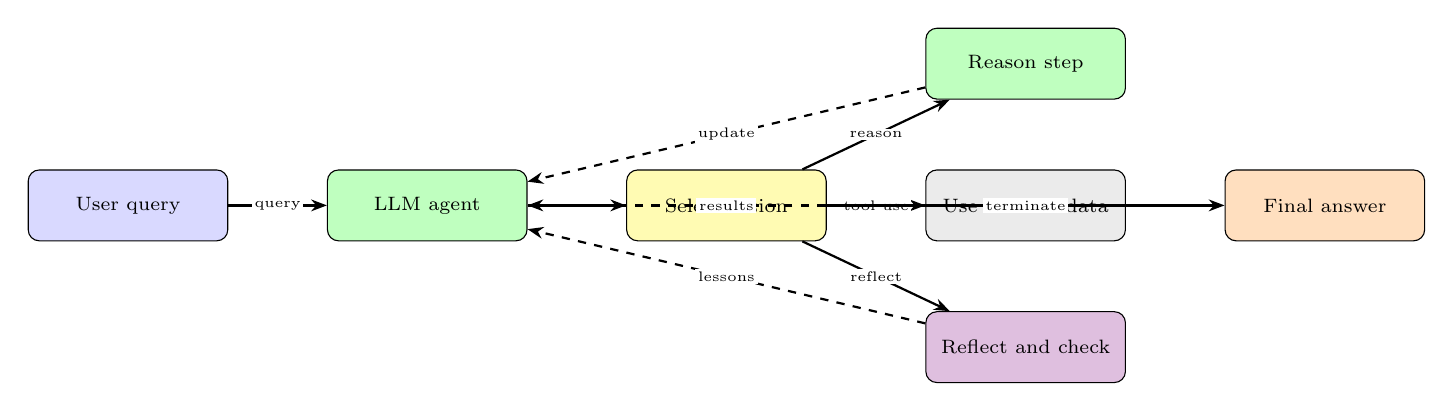
\begin{tikzpicture}
    \node[kuser] (user) at (0.00,0.00) {User query};
    \node[kagent] (agent) at (3.80,0.00) {LLM agent};
    \node[kdecision] (decide) at (7.60,0.00) {Select action};
    \node[kagent] (reason) at (11.40,1.80) {Reason step};
    \node[kdata] (tool) at (11.40,0.00) {Use tools or data};
    \node[kguard] (reflect) at (11.40,-1.80) {Reflect and check};
    \node[koutput] (output) at (15.20,0.00) {Final answer};
    \draw[flow] (user) -- (agent) node[midway, font=\tiny, fill=white, inner sep=1pt]{query};
    \draw[flow] (agent) -- (decide);
    \draw[flow] (decide) -- (reason) node[midway, font=\tiny, fill=white, inner sep=1pt]{reason};
    \draw[flow] (decide) -- (tool) node[midway, font=\tiny, fill=white, inner sep=1pt]{tool use};
    \draw[flow] (decide) -- (reflect) node[midway, font=\tiny, fill=white, inner sep=1pt]{reflect};
    \draw[flow, dashed] (reason) -- (agent) node[midway, font=\tiny, fill=white, inner sep=1pt]{update};
    \draw[flow, dashed] (tool) -- (agent) node[midway, font=\tiny, fill=white, inner sep=1pt]{results};
    \draw[flow, dashed] (reflect) -- (agent) node[midway, font=\tiny, fill=white, inner sep=1pt]{lessons};
    \draw[flow] (decide) -- (output) node[midway, font=\tiny, fill=white, inner sep=1pt]{terminate};
  \end{tikzpicture}%
  }
  \end{center}
  \begin{center}\scriptsize The general agentic reasoning loop: an agent repeatedly reasons, uses tools, or reflects until it produces a final answer.\end{center}
\end{frame}
\note{This diagram shows the general loop that ties everything together. A user sends a query, the agent reads it, and then picks one action: reason, use a tool, or reflect. Each action updates what the agent knows and loops back around. When the goal is met, the agent stops and returns the final answer.}
\begin{frame}[allowframebreaks]{How It Works (Explained)}
\begin{itemize}
  \item A user sends a query into the agent as the starting input
  \item The LLM agent reads the query and its current context
  \item It then selects one action from its action space
  \item Reason expands the thinking, tool-use fetches data, reflect self-checks
  \item Each action updates the context and loops back to the agent
  \item When the goal is met, the agent returns the final answer
\end{itemize}
\end{frame}
\section{Example Walkthrough}
\begin{frame}[allowframebreaks]{Example Walkthrough: Fixing a Bug with a Coding Agent}
\begin{enumerate}
  \item User asks the agent to fix a failing function
  \item Agent reasons about why the test might be failing
  \item Agent calls a tool to run the code and read the error
  \item Using the error, it reasons about the correct fix
  \item Agent edits the code and runs the tests again
  \item Reflection checks whether all tests now pass
  \item Agent returns the fixed, verified code to the user
\end{enumerate}
\end{frame}
\note{Let's make this concrete with a coding example. Imagine you ask the agent to fix a broken function. It reasons about the likely cause, runs the code as a tool to see the real error, fixes it, and runs the tests again. It reflects to confirm everything passes, then hands back the corrected code. That single example uses reasoning, tools, and reflection all together.}
\section{Results}
\begin{frame}[allowframebreaks]{Results / Findings}
\begin{itemize}
  \item Survey spans 51 pages with 10 figures and 8 tables
  \item Organizes agent reasoning into 3 main framework families
  \item Single-agent, tool-based, and multi-agent each split into subtypes
  \item Covers 5-plus scenarios: science, healthcare, software, social, economics
  \item Reviews benchmarks like GSM8K, HumanEval, MBPP, MMLU, and MATH
  \item Proposes 6 future research directions for the field
\end{itemize}
\end{frame}
\note{Since this is a survey, the results are really about coverage and organization. The paper spans fifty-one pages with ten figures and eight tables. It sorts agents into three families, connects them to five or more real domains, reviews well-known benchmarks like GSM8K and HumanEval, and lays out six directions for future work.}
\section{Discussion}
\begin{frame}{Discussion}
\begin{itemize}
  \item No single framework wins; the best choice depends on the task
  \item Simple tasks suit single agents; complex ones benefit from tools or teams
  \item More agents add power but also cost and coordination overhead
  \item Framework design matters as much as raw model strength
\end{itemize}
\end{frame}
\note{The big takeaway from the discussion is that there's no single best framework. A simple question might only need one agent, while a complex project benefits from tools or a whole team of agents. But adding agents also adds cost and coordination headaches, so design choices really matter.}
\section{Challenges}
\begin{frame}{Limitations \& Challenges}
\begin{itemize}
  \item LLMs still hallucinate and can rely on outdated knowledge
  \item Tool selection depends heavily on clear tool descriptions
  \item Iterative optimization may settle on suboptimal solutions
  \item Centralized multi-agent setups can create performance bottlenecks
\end{itemize}
\end{frame}
\note{It's important to be honest about the weak spots. These agents can still hallucinate or rely on outdated knowledge. Tool use only works well when tools are clearly described, self-improvement can get stuck on a mediocre answer, and central coordinators can become bottlenecks.}
\section{Future Work}
\begin{frame}{Future Work}
\begin{itemize}
  \item Improve scalability and reduce the cost of reasoning
  \item Enable open-ended, self-directed autonomous learning
  \item Strengthen reliability, safety, ethics, and fairness
  \item Add confidence estimation and clearer explainability
\end{itemize}
\end{frame}
\note{Looking ahead, the authors highlight a few frontiers. We need agents that are cheaper and more scalable, that can learn on their own, and that we can trust to be safe, fair, and reliable. They also want agents that can express how confident they are and explain their reasoning.}
\section{Conclusion}
\begin{frame}{Conclusion}
\begin{itemize}
  \item Agentic reasoning frameworks turn LLMs into capable problem-solvers
  \item A unified taxonomy clarifies single-agent, tool-based, and multi-agent design
  \item Matching the framework to the scenario is key to performance
  \item Framework innovation, beyond bigger models, will drive future agents
\end{itemize}
\end{frame}
\note{To wrap up: agentic reasoning frameworks are what turn a plain language model into a real problem-solver. This survey gives us a clean map of single-agent, tool-based, and multi-agent designs, and reminds us that matching the framework to the task is what really matters. Thanks, and I'm happy to take questions.}
\section{References}
\begin{frame}[allowframebreaks]{References}
  \footnotesize
  \begin{enumerate}
    \item Zhao, B., Foo, L. G., Hu, P., Theobalt, C., Rahmani, H., \& Liu, J. (2025). LLM-based Agentic Reasoning Frameworks: A Survey from Methods to Scenarios. arXiv:2508.17692.
    \item Yao, S., Zhao, J., Yu, D., Du, N., Shafran, I., Narasimhan, K., \& Cao, Y. (2023). ReAct: Synergizing Reasoning and Acting in Language Models. ICLR 2023. arXiv:2210.03629.
    \item Shinn, N., Cassano, F., Berman, E., Gopinath, A., Narasimhan, K., \& Yao, S. (2023). Reflexion: Language Agents with Verbal Reinforcement Learning. NeurIPS 2023. arXiv:2303.11366.
    \item Hong, S., Zheng, M., Chen, J., et al. (2024). MetaGPT: Meta Programming for a Multi-Agent Collaborative Framework. ICLR 2024. arXiv:2308.00352.
    \item Wu, Q., Bansal, G., Zhang, J., et al. (2023). AutoGen: Enabling Next-Gen LLM Applications via Multi-Agent Conversation. arXiv:2308.08155.
    \item Madaan, A., Tandon, N., Gupta, P., et al. (2023). Self-Refine: Iterative Refinement with Self-Feedback. NeurIPS 2023. arXiv:2303.17651.
  \end{enumerate}
\end{frame}
\begin{frame}[plain]
  \begin{center}
    {\Huge Thank You}\\[1em]
    {\large Questions?}
  \end{center}
\end{frame}
\end{document}